\section{Существующие решения}\label{ch:--}
\subsection{Обзор методов модификации ядра Linux}\label{sec:----linux}

В данном разделе рассмотрены основные методы модификации ядра Linux, которые используются в настоящее время.
Все они различаются по своим особенностям и применяемым технологиям.

\subsubsection{Методы модификации ядра Linux, основанные на перекомпиляции ядра}\label{subsec:---linux----}

На момент выпуска версии 1.0 ядра Linux существовал единственный метод модификации ядра Linux, основанный на перекомпиляции ядра.
В этом методе исходный код Linux изменяется под конкретные задачи и перекомпилируется с использованием специальных опций компилятора.
В результате получается модифицированное ядро Linux, которое можно использовать для запуска системы.
Однако, такой метод модификации ядра Linux имеет ряд недостатков:
\begin{enumerate}
    %FIXME
    \item Необходимость перекомпиляции ядра Linux для каждого нового модуля. \vspace{1mm}\\
    Это означает, что при необходимости добавления нового модуля в систему необходимо будет внести нужные изменения и перекомпилировать все ядро Linux, что влечет за собой массу проблем.
    Так, например, при перекомпиляции ядра необходима полная остановка системы и таким образом этот метод модификации ядра не подходит для систем, в которых необходимо добавлять новые модули динамически.

    \item Сложность добавления кода в ядро Linux. \vspace{1mm}\\
    Для добавления кода в ядро Linux необходимо уметь работать с языком и компилятором языка C, а также с инструментами конфигурации ядра Linux, знать интерфейс прикладного программирования ядра (API)\cite{API-linux}.
    Иными словами данный подход требует крайне высокой квалификации команды разработчиков, что замедляет процесс разработки и внедрения новых модулей в систему.
    \item В случае если при добавлении нового кода в ядро Linux была допущена ошибка, то есть шанс повредить систему и сделать её полностью нерабочей.
\end{enumerate}

Однако у статического метода модификации ядра Linux есть и преимущества:

\begin{enumerate}
    \item Скорость работы системы. \vspace{1mm}\\
    В статическом методе модификации ядра Linux не используется динамическая загрузка модулей, поэтому модули ядра Linux загружаются в память только один раз, при запуске системы.
    Поэтому, в статическом методе модификации ядра Linux исключена возможность динамического добавления новых модулей в систему, что позволяет увеличить скорость работы системы.
    \item Отсутствие альтернативных методов модификации ядра Linux.\vspace{1mm}\\
    Иногда необходимые дополнения не могут быть реализованы в виде модулей ядра Linux, поэтому в этом случае необходимо модифицировать исходный код ядра Linux.
    \item В версии ядра 6.1 была добавлена поддержка языка Rust, что частично нивелировало сложность написания кода для ядра, поскольку данный язык дает разработчикам возможность написания высокоуровневого кода без потери производительности системы.
\end{enumerate}

\subsubsection{Методы модификации ядра Linux, основанные на встраивании модулей ядра}\label{subsec:---linux-----}

Второй метод модификации ядра Linux, основанный на встраивании модулей ядра, появился в 1995 году, когда в версию 1.2 была добавлена поддержка LKM - Loadable Kernel Module.
В этом методе ядро Linux не перекомпилируется.
Вместо этого используется специальный модуль ядра, который встраивается в ядро Linux.
В результате получается модифицированное ядро Linux, которое можно использовать для работы системы.

\begin{figure}[H]
    \centering
    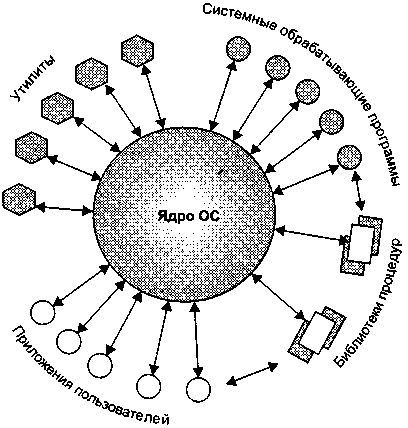
\includegraphics[width=105mm, scale=0.65]{inc/img/lkm}
    \caption{Взаимодействие ядра с загружаемыми модулями и пользовательскими приложениями.}
    \label{fig:lkm}
\end{figure}

В качестве примера можно привести модуль ядра, который предназначен для работы с сетевыми интерфейсами.
В этом модуле ядра реализованы функции, которые позволяют получить информацию о сетевых интерфейсах, а также управлять ими.
При этом, модуль ядра не содержит в себе никаких функций, которые не относятся к работе с сетевыми интерфейсами.
Таким образом, модуль ядра не засоряет ядро Linux ненужными функциями.
\vspace{1mm}\\
\textbf{Плюсы:}

\begin{enumerate}
    \item Модуль ядра может быть загружен в ядро Linux во время работы системы. \vspace{1mm}\\
    Таким образом, система может продолжать работать, динамически меняя свою конфигурацию по мере необходимости.
%    \item Модифицированное ядро Linux является частью исходного кода ядра Linux. %\vspace{1mm}\\
%    Поэтому, если в исходный код ядра Linux вносятся изменения, то исходный код модифицированного ядра Linux автоматически изменяется.
    \item Модуль ядра может сэкономить оперативную память,
    потому что появляется возможность загружать их только тогда, когда они действительно нужны, в то время как
    все части базового ядра все время остаются загруженными в реальном хранилище, а не только в виртуальном.
    \item Еще одним преимуществом LKM является то, что он помогает диагностировать системные проблемы. \vspace{1mm}\\
    Ошибка в драйвере устройства, связанном с ядром, может остановить загрузку системы, что может вызвать проблемы определить, какая часть базового ядра вызвала проблемы.
    Однако если тот же драйвер устройства будет загружен в систему динамически, то базовое ядро способно запуститься и продолжать работу еще до загрузки драйвера устройства.
    Если система завершает работу после того, как базовое ядро было запущено, то появляется возможность отследить проблему до вызывающего проблемы драйвера устройства и не загружать его до тех пор, пока проблема не будет решена.
\end{enumerate}

\textbf{Недостатки:}
\begin{enumerate}
    \item LKM может привести к проблемам с производительностью системы. \vspace{1mm}\\
    Поскольку LKM загружаются в ядро Linux во время работы системы, они могут увеличить время загрузки системы.
    \item В некоторых случаях LKM может привести к некоторым системным проблемам. \vspace{1mm}\\
    Например, LKM может привести к проблемам совместимости, если они не совместимы с базовым ядром.
    \item Еще одним из незначительных критических замечаний по поводу предпочтения модульного ядра статическому ядру является так называемый штраф за фрагментацию. \vspace{1mm}\\
    Базовое ядро всегда распаковывается в реальную непрерывную память своими программами установки;
    таким образом, базовый код ядра никогда не фрагментируется.
    Как только система находится в состоянии, в котором модули могут быть вставлены, например, после того, как были смонтированы файловые системы, содержащие модули, вполне вероятно,
    что любая новая вставка кода ядра приведет к фрагментации ядра, что приведет к незначительному снижению производительности.
    \item Так же как и при добавлении кода напрямую в ядро, если при работе модуля возникнет ошибка, то есть шанс, что система также экстренно завершит работу.
\end{enumerate}

\subsubsection{Kernel Live Patching}\label{subsec:kernel-live-patching}

Kernel Live Patching - это функция ядра Linux, которая позволяет обновлять ядро Linux без перезагрузки системы.
Первая программная реализация данной идеи принадлежит команде Джеффа Арнольда, студентов MIT, носит название Ksplice\cite{ksplice}, а её первая коммерческая версия была запущена в 2010 году.
Исправление ядра в реальном времени является важным компонентом стратегии управления серверами Linux и устранения уязвимостей.
\\
Принцип Live Patching'а основан на том, что данный метод модификации ядра создает отдельный модуль из исправленного кода, а затем с помощью инструмента ftrace (трассировки функций) перенаправляет вызов от устаревшей функции к новой.
На рисунке \ref{fig:Livepatch} показана схема работы данного метода.

\begin{figure}[H]
    \centering
    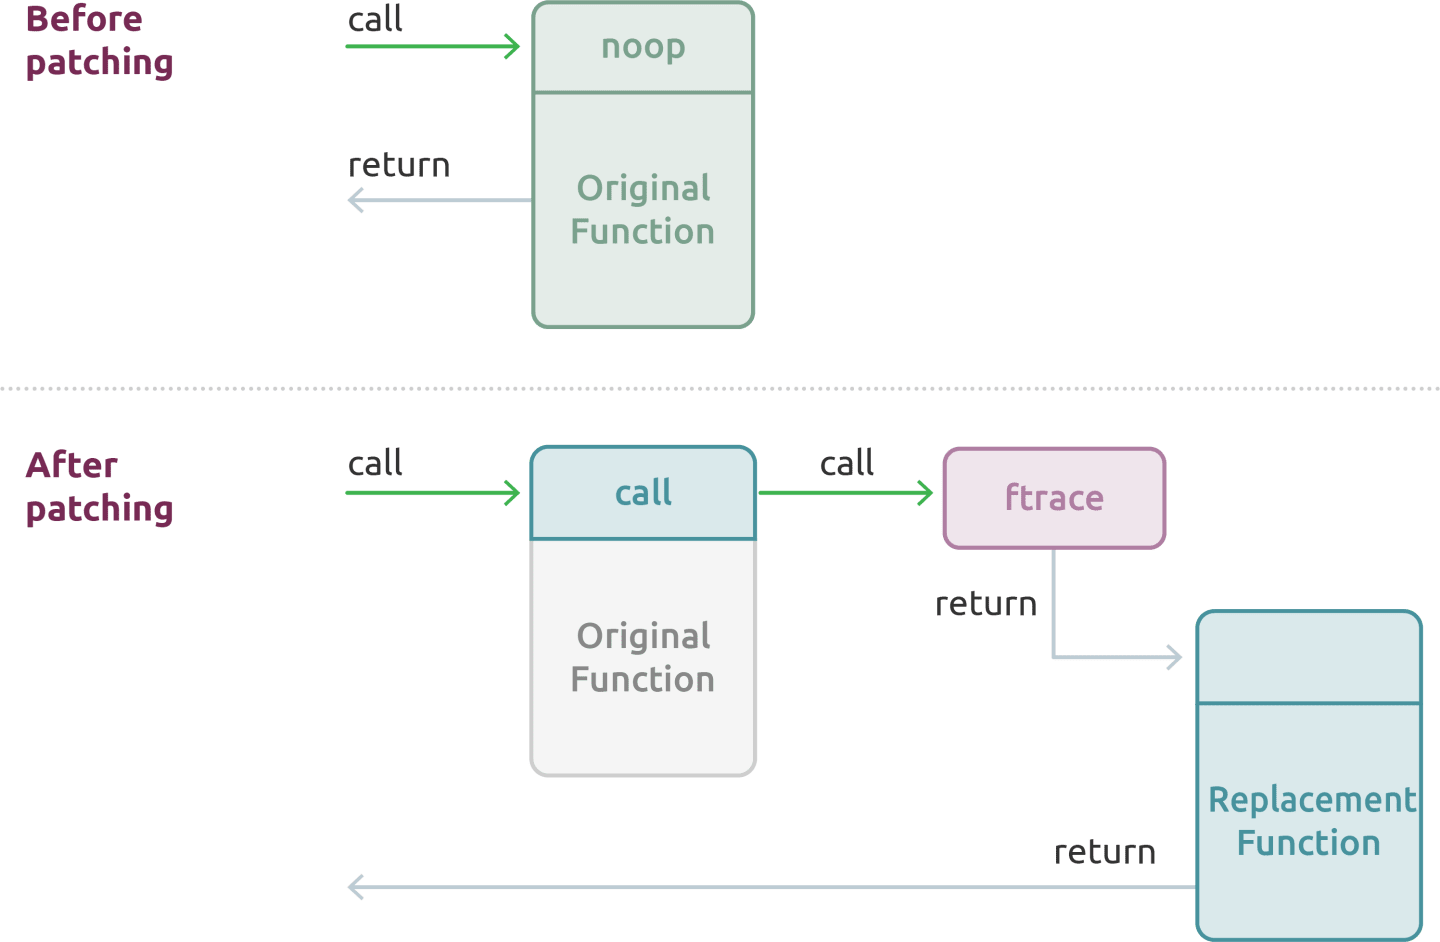
\includegraphics[scale=0.75, width=\textwidth]{inc/img/Livepatch}
    \caption{Концепт Live Patching.}
    \label{fig:Livepatch}
\end{figure}

\textbf{Преимущества:}

\begin{enumerate}
    \item Позволяет обновлять ядро Linux без перезагрузки системы.
    \item Обновление системы требует времени и высокого уровня навыков системного администрирования.
    Live Patching избавляет персонал от рутинной работы по рутинному обслуживанию многочисленных серверов.
    \item Обновления проходят быстро, что позволяет оперативное разворачивание новых функций.
\end{enumerate}

\textbf{Недостатки:}

\begin{enumerate}
    \item Внесение исправлений в ядро по-прежнему сложно — исправления должны быть написаны экспертами для каждой системы,
    и они зарезервированы только для важных исправлений безопасности.
    Даже в этом случае не гарантируется, что система не выйдет из строя.
    Так например различные оптимизации при компиляции могут незаметно изменить код таким образом, что это может привести к серьезным проблемам при применении исправления.\cite{livepatch-problems}
    \item Live Patching может применяться только к небольшим и конкретным частям кода ядра и не может использоваться для каких-либо серьезных обновлений,
    которые затрагивают несколько компонентов или изменяют структуры данных.
    \vspace{0.5cm}\\
    Изменения в структурах данных усложняют ситуацию, поскольку данные должны оставаться на месте и не могут быть расширены или переинтерпретированы.
    Хотя существуют методы, которые позволяют косвенно изменять структуры данных, некоторые изменения нельзя преобразовать в подобного рода исправления.
    В этой ситуации перезагрузка системы — единственный способ применить все изменения.
    \item Не все ядра поддерживают Live Patching.
    В различных ядрах используются разные методы управления процессом исправления и создания исправлений,
    а некоторые из них разработаны исключительно под определенные семейства Linux.\cite{infosec}
\end{enumerate}

\subsubsection{eBPF}\label{subsec:ebpf}

eBPF (extended Berkeley Packet Filter) - это новая технология, которая позволяет встраивать программы в ядро Linux, не изменяя его исходный код.
В своей основе eBPF использует привилегированную способность ядра видеть и контролировать все ресурсы системы.
С помощью eBPF есть возможность запускать изолированные программы в привилегированном контексте, которые могут взаимодействовать с ядром Linux.

\begin{figure}[H]
    \centering
    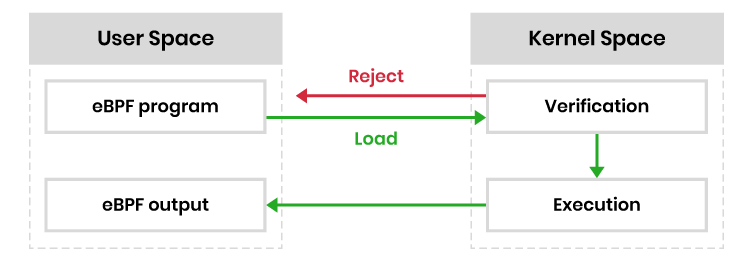
\includegraphics[width=\textwidth]{inc/img/eBPF_work}
    \caption{Алгоритм eBPF.}
    \label{fig:eBPF_work}
\end{figure}

%\vspace{1mm}\\

eBPF работает по следующему принципу:\\%\vspace{0.5cm}}

eBPF позволяет приложениям пространства пользователя упаковывать логику, которая будет выполняться в ядре Linux, в виде байт-кода.
eBPF-программы вызываются ядром, когда происходят определенные события, называемые <<системными хуками>>.
Примеры таких событий включают в себя системные вызовы, сетевые события и т.д.\\
Перед загрузкой в ядро eBPF-программа должна пройти определенный набор проверок со стороны так называемого верификатора.
Только если все проверки пройдены успешно, программа eBPF преобразуется в байт-код, загружается в ядро и начинает ждать соответствующих ей событий.
После того, как событие произошло, eBPF-программа выполняется в привилегированном контексте ядра.

\textbf{Преимущества:}

\begin{enumerate}
    \item eBPF позволяет встраивать программы в ядро Linux, не изменяя его исходный код.
	    В то время как все остальные методы вносят дополнительные факторы риска в работоспособность системы, eBPF с данной точки зрения абсолютно безопасен.
        Все программы перед компиляцией проходят строгую проверку со стороны одного из собственных модулей eBPF, так называемого верификатора, в следствии чего можно быть уверенным в безопасности исполняемого кода.
    \item eBPF позволяет писать программы на различных высокоуровневых языках, что значительно упрощает процесс разработки.
    Данная возможность обеспечивается с помощью компилятора LLVM, который позволяет компилировать код на различных языках в байт-код, который затем исполняется виртуальной машиной eBPF.
    \item Также как и LKM, eBPF позволяет динамически загружать и выгружать программы во время работы системы. %\vspace{1mm}\\
    Поскольку eBPF является JIT-компилятором, то он может компилировать программы в машинный код на лету, что позволяет изменять конфигурацию системы в реальном времени.
\end{enumerate}

\textbf{Недостатки:}

\begin{enumerate}
    \item Главный минус eBPF заключается в том, что количество функций, которыми программист может манипулировать, сильно ограничено.\\
    eBPF обеспечивает повышенную безопасность, ограничивая доступ программ к ресурсам системы.
    Однако из-за такого ограничения, к каким частям ОС программа может получить доступ, функциональность данного метода также ограничена.
    \item Подобно LKM, в случае если необходимо внести изменения в уже загруженные в ядро функции, то eBPF просто не обладает данной возможностью.
    \item Поскольку eBPF выполняет программы в привилегированном контексте, то это может привести к утечке конфиденциальной информации.
    Исторически eBPF обладает множеством уязвимостей, которые могут быть использованы для получения нежелательного доступа к критическим ресурсам системы.
    Примером одной из таких уязвимостей является CVE-2021-4204\cite{cve-2021-4204}, которая позволяет произвольному непривилегированному пользователю получить доступ к памяти ядра.
    \item eBPF является молодым и пока еще развивающимся инструментом.
    В связи с этим в ходе разработки eBPF-программ могут возникать проблемы, связанные с отсутствием документации или её недостаточной информативностью.
\end{enumerate}
\newpage
\noindent В конце данного раздела стоит сделать оговорку касательно eBPF\@.
\vspace{5mm}\\
eBPF де-факто не является полноценным инструментом модификации ядра.\\
eBPF — это всего лишь набор инструкций, для которых ядро Linux предоставляет виртуальную машину, верификатор и некоторые вспомогательные функции.
Программы запускаются внутри этого контекста выполнения и вызывают вспомогательные функции для расширения возможностей виртуальной машины.
Во время выполнения программы eBPF на самом деле вызываются kprobe, или uprobe, или классификатор eXpress Data Path (XDP),
или один из многих других типов программ пространства ядра, которые были выгружены в подсистему eBPF\@.
\\
Таким образом, eBPF-программы — это не полноценные модификации ядра Linux, а лишь наборы инструкций, которые позволяют расширить возможности уже существующего модуля ядра\@.
Но не смотря на это, по формальным признакам, eBPF подходит под все критерии, которые были описаны в начале данной работы,
являясь при этом крайне мощным инструментом при написании определенного типа программ, что и послужило причиной для его включения в данную работу.
\newpage

\subsection{Критерии сравнения методов модификации ядра}\label{sec:----}
В данном разделе будут описаны критерии, которые будут использоваться для сравнения методов модификации ядра.

\begin{table}[ht]
\begin{center}
    \begin{threeparttable}
      \captionsetup{justification=raggedright,singlelinecheck=off}
      \caption{\label{tab:criteria}Критерии сравнения методов модификации ядра}
        \begin{tabular}{|c|p{8cm}|}
        \hline
        \textbf{Критерий} & \textbf{Описание} \\ \hline
        \textbf{Производительность} & Производительность программ. \\ \hline
        \textbf{Безопасность} & Наличие гарантии, что внесенный код не вызовет остановку системы. \\ \hline
        \textbf{Скорость разработки} & Скорость разработки модификации. \\ \hline
        \textbf{Гибкость} & Возможность метода подстроиться под любые поставленные бизнес-задачи. \\ \hline
        \textbf{Простота отладки} & Является ли описанная модификация простой в отладке. \\ \hline
        %\textbf{Кроссплатформенность} & Возможность использования модификаций на разных архитектурах. \\ \hline
        \textbf{Поддержка} & Поддержка метода разработчиками ядра при его написании. \\ \hline
        \textbf{Простота развёртывания} & Является ли описанный метод простым в развёртывании на большом количестве машин. \\ \hline
        \end{tabular}
    \end{threeparttable}
\end{center}
\end{table}
\newpage
\subsection{Сравнение методов модификации ядра}\label{sec:---}
% \textbf{TODO: добавить комментарии к сравнению}
% cmark and xmark defined in research.tex
В данном разделе будут описаны все описанные в работе методы модификации ядра, а также будет дано сравнение этих методов по всем критериям, указанным в таблице~\ref{tab:criteria}.

\begin{table}[ht]
\begin{center}
    \begin{threeparttable}
        \captionsetup{justification=raggedright,singlelinecheck=off}
        \caption{\label{tab:comparison} Сравнение методов модификации ядра}
        \begin{tabular}{|c|c|c|c|c|}
            \hline
            \textbf{Критерий} & \textbf{Рекомпиляция} & \textbf{LKM} & \textbf{Live Patching} & \textbf{eBPF} \\ \hline
            \textbf{Производительность} & \cmark & \cmark & \cmark & \cmark \\ \hline
            \textbf{Безопасность} & \xmark & \xmark & \xmark & \cmark \\ \hline
            \textbf{Скорость разработки} & \xmark & \cmark & \xmark & \cmark \\ \hline
            \textbf{Гибкость} & \cmark & \cmark & \xmark & \xmark \\ \hline
            \textbf{Простота отладки} & \xmark & \cmark/\xmark\footnotemark & \xmark & \cmark \\ \hline
%            \textbf{Кроссплатформенность} & \cmark & \cmark/\xmark & \cmark & \cmark \\ \hline
            \textbf{Поддержка} & \cmark & \cmark & \cmark & \xmark \\ \hline
            \textbf{Простота развёртывания} & \xmark & \cmark & \cmark & \cmark \\ \hline
        \end{tabular}
    \end{threeparttable}
\end{center}
\end{table}

\footnotetext{Несмотря на то, что в данном методе отладка происходит гораздо легче, чем при встраивании кода в само ядро, как при рекомпиляции или Live Patching'е, отладка модулей всё равно может вызвать ряд проблем.}

Полученные результаты можно свести к следующему:
\begin{itemize}
    \item[--] Рекомпиляция ядра -- самый гибкий метод, но самый сложный в развёртывании и отладке, а также требующий большего времени на разработку.
    Также, рекомпиляция ядра требует перезагрузки системы, что может быть нежелательно в некоторых случаях.
    \item[--] LKM -- второй по гибкости метод модификации ядра, однако, в отличие от рекомпиляции, не требует перезагрузки системы.
    Тем не менее LKM разделяет частично проблемы рекомпиляции ядра: медленная разработка, относительная сложность отладки, а также риск остановки системы при неправильной работе модуля.
    \item[--] Live Patching -- крайне ограниченный метод модификации ядра, который позволяет вносить изменения в ядро только в определённых случаях, чаще всего в виде исправления ошибок.
    Однако, он позволяет вносить изменения в уже загруженные функции ядра, без перезагрузки системы, что является большим плюсом.
    \item[--] eBPF -- самый простой и быстрый метод модификации ядра, однако, он ограничен в своих возможностях.
    Так например, eBPF не имеет возможности применять политики доступа к системным вызовам.
    Таким образом нельзя запретить пользователю открывать какой-либо файл, используя инструментарий eBPF\@.
    Взамен этому он предоставляет безопасный и высокопроизводительный способ выполнения кода на уровне ядра.
\end{itemize}

\indent Из результатов сравнения было выявлено, что каждый из методов модификации ядра Linux различен относительно других методов по своим преимуществам и недостаткам.
Таким образом, выбор метода модификации ядра Linux зависит в первую очередь от конкретных задач, которые необходимо решить, и нет единого метода, который был бы наилучшим для решения всех задач.
Разработанная в ходе работы методика позволяет сравнивать методы модификации ядра Linux и определять, какой из методов подходит для решения конкретной задачи.
